\documentclass[final]{beamer}
\usefonttheme[onlymath]{serif}
\usepackage{subfig}
\usepackage{xcolor}
\usepackage[utf8]{inputenc}
\usetheme{SUPoster}
\usepackage{multicol}
\usepackage{diagbox}
\usepackage{tabularx}
\usepackage{booktabs}
\usepackage{todonotes}

%\usepackage[demo]{graphicx}
\usepackage{caption}
\usepackage{subcaption}

\usepackage{multirow}


\usepackage[orientation=landscape,size=a1,scale=1.6]{beamerposter}

\captionsetup[figure]{labelformat=empty}% redefines the caption setup of the figures environment in the beamer class.
%\captionsetup[subfigure]{labelformat=empty}
\usepackage[absolute,overlay]{textpos}
\setlength{\TPHorizModule}{1cm}
\setlength{\TPVertModule}{1cm}


\usepackage{lmodern} % needed to make math mode fonts scale properly
\usepackage{url}
\usepackage{graphics}
\usepackage{bold-extra}
\usepackage{movie15}
\usepackage{caption}

\usepackage{enumitem}
% \setitemize[1]{label=$\blacktriangleright$}
% \setlist[itemize,1]{label=$\blacktriangleright$}

\setlist[itemize]{label=\usebeamerfont*{itemize item}%
  \usebeamercolor[fg]{itemize item}
  \usebeamertemplate{itemize item},
  leftmargin=1em}

% next line is necessary to make beamer and enumitem play nicely together (see http://tex.stackexchange.com/questions/45921/make-enumerate-have-beamer-themes-when-using-enumitem/45950#45950)
\setlist[enumerate]{leftmargin=2.2em,%
label=\protect\usebeamerfont{enumerate item}%
    \protect\usebeamercolor[fg]{enumerate item}%
    \insertenumlabel. }

%% DOCUMENT DATA

\title{A Formal Methods Approach Towards Deep Learning Interpretability}

\author{Kristen Kessel, Christopher Lazarus, Javier Sagastuy}
\institute{Stanford University}

\logoleft{\begin{center} 
\includegraphics[height=4.5cm]{img/SU_Seal_Blk_pos}\end{center}}
\logoright{\begin{center} 
\includegraphics[height=4.5cm]{img/icme_logo_trans} \end{center}}
\footer{CS 231N $|$ Spring 2019 \hspace{38cm} \{\texttt{kkessel, clazarus, jvrsgsty}\}\texttt{@stanford.edu}}
%
%\date{}

\begin{document}


\definecolor{almostWhite}{RGB}{240,240,240}
\definecolor{lightGray}{RGB}{220,220,220}
\definecolor{tbllinecolor}{RGB}{200,200,200}
\beamertemplateshadingbackground{lightGray}{almostWhite}
\newcommand{\vltbl}{{\color{tbllinecolor}\vrule}}


\begin{frame}[fragile]{}

%%%%%%%%%%%%%%%%%%%%%%%%%%%%%%%%%%%%%%%%%%%%%%%%%%%%%%%%%%%%%%%%%%%%
% IMPORTANT:
%   Here is where you define your poster's layout params (widths and
%   vertical positions).
%   Feel free to add/remove more, to make your layout fit your needs
%
%   All dimensions are in cm (I think).
%%%%%%%%%%%%%%%%%%%%%%%%%%%%%%%%%%%%%%%%%%%%%%%%%%%%%%%%%%%%%%%%%%%%

% centralize columns layout
\newcommand{\vstart}{58} % where the top row start vertically
\newcommand{\vstartCols}{8} % where the columns start vertically
\newcommand{\fullwidth}{81}  % this is the key to the values below
\newcommand{\colwidth}{26.5}

\newcommand{\firstcolpos}{1}
\newcommand{\secondcolpos}{28.75}
\newcommand{\thirdcolpos}{56.5}
\newcommand{\bottomblockstart}{108.5}


% this will add some padding to the blocks, to avoid text reaching
% the border (looks bad)
\newenvironment{paddedBlock}[2][0.95\linewidth]
    {\begin{block}{#2}\begin{minipage}{#1}}
    {\end{minipage}\end{block}}

%%%%%%%%%%%%%%%%%%%%%%%%%%%%%%%%%%%%%%%%%%%%%%%%%%%%%%%%%%%%%%%%%%%%
% And now ... the content
%%%%%%%%%%%%%%%%%%%%%%%%%%%%%%%%%%%%%%%%%%%%%%%%%%%%%%%%%%%%%%%%%%%%

%%%%%%%%%%%%%%%%%%%%%%%%%
%%%%%%%%%%%%%%%%%%%%%%%%%
%% LEFT COLUMN
%%%%%%%%%%%%%%%%%%%%%%%%%
%%%%%%%%%%%%%%%%%%%%%%%%%
\begin{textblock}{\colwidth}(\firstcolpos,\vstartCols)

\begin{paddedBlock}{Summary}
Although deep neural networks have proved to be very successful at classification tasks, their intrinsic complexity makes reasoning about a classification outcome difficult.
In recent work [2], statistical methods were introduced as a means to quantify the influence of human-intelligible concepts in classification outcomes.
We aim to assess and extend such methods by leveraging formal methods for neural network verification.
\begin{itemize}
\item \textbf{Question:} How important is a concept in classifying image $i$ as label $k$? e.g. Is the presence of stripes relevant in the classification of an animal as a zebra?
\item \textbf{Approach \#1:} Use the TCAV framework to provide statistical guarantees
\item \textbf{Approach \#2:} Use neural network verification methods [1] to provide formal guarantees
\end{itemize}
\end{paddedBlock}

\begin{paddedBlock}{Testing with Concept Activation Vectors (TCAV) [2]}
\begin{itemize}
\item \textbf{Idea:} \footnotesize{Identify the region in the latent space corresponding to layer $\ell$ of the network in which a concept (e.g. blue) manifests more intensely with a vector called the Concept Activation Vector (CAV). Measure the relevance of this concept for classification of image $i$ as class $k$ by taking directional derivative of the layer $\ell$ activations for image $i$ with respect to the CAV.}
\end{itemize}
\begin{itemize}
\item \textbf{Inputs:}
	\begin{itemize}
	\footnotesize{
	\item trained classification network
	\item set of examples for a user-defined concept $C$ and set of random counterexamples
    \item labeled examples for the class $k$ under consideration
    }
	\end{itemize}
\item \textbf{Outputs:}
	\begin{itemize}
	\footnotesize{
	\item CAV $v_c^\ell$ for concept $C$ at layer $\ell$
    \item score $S_{C,k}^\ell(\mathbf{x})$ of the sensitivity of the model's prediction of class $k$ to concept $C$
    	\[ S_{C,k}^\ell(\mathbf{x}) = \nabla h_k^\ell\left(f_\ell(\mathbf{x})\right) \cdot \mathbf{v}_C^\ell \]
    \item TCAV score aggregating scores for each training image $\mathbf{x}$ in class $X_k$
    	\[ \text{TCAV}_{C, k}^\ell = \frac{\left| \mathbf{x} \in X_k : S_{C,k}^\ell(\mathbf{x}) > 0 \right|}{\left| X_k \right|} \]
    \item $p$-value testing the hypothesis that concept $C$ is not relevant in classifying images of class $k$
    }
	\end{itemize}
\end{itemize}
%\vspace{-5mm}
\end{paddedBlock}

\begin{paddedBlock}{Neural Network Verification}

For input set $\mathcal{X}$, neural network $f$, and output set $\mathcal{Y}$, we seek to verify statements of the following form:
\[ \vec x\in \mathcal{X} \Rightarrow \vec y=\vec f(\vec x)\in \mathcal{Y} \]
\end{paddedBlock}
\end{textblock}

%%%%%%%%%%%%%%%%%%%%%%%%%
%%%%%%%%%%%%%%%%%%%%%%%%%
%% RIGHT COLUMN
%%%%%%%%%%%%%%%%%%%%%%%%%
%%%%%%%%%%%%%%%%%%%%%%%%%
\begin{textblock}{\colwidth}(\secondcolpos,\vstartCols)
\begin{paddedBlock}{Approach \#1: TCAV}
%\vspace{8mm}

\alert{Custom Data Sets}
%\begin{figure}%
%    \centering
%    \subfloat[label 1]{{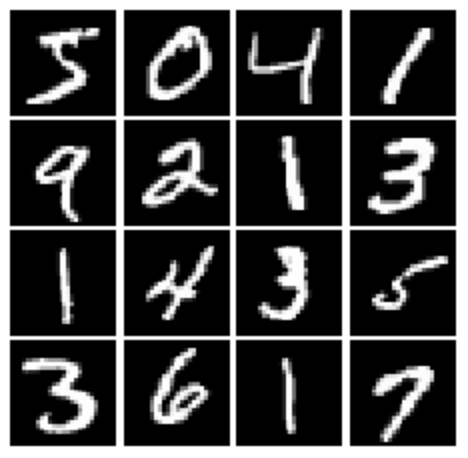
\includegraphics[width=5cm]{img/mnist_bw.png} }}%
%    \qquad
%    \subfloat[label 2]{{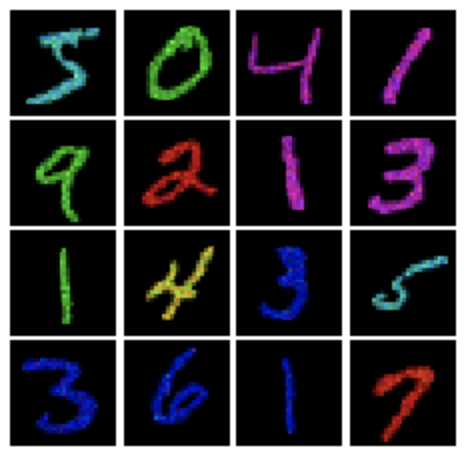
\includegraphics[width=5cm]{img/mnist_color.png} }}%
%    \caption{2 Figures side by side}%
%    \label{fig:example}%
%\end{figure}

\begin{figure}%
    \centering
    \subfloat{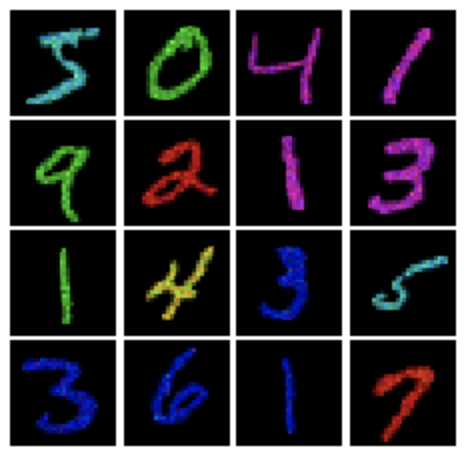
\includegraphics[width=.2\textwidth]{img/mnist_color.png}}}%
    \qquad
    \subfloat{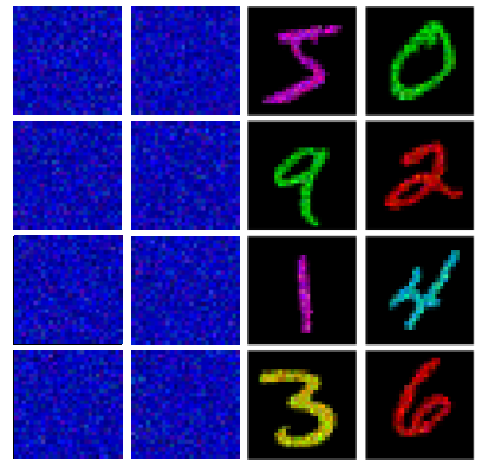
\includegraphics[width=.2\textwidth]{img/cav_viz2}}}%
    \qquad
    \subfloat{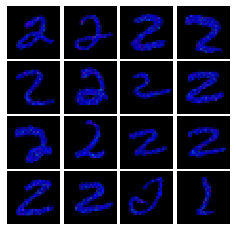
\includegraphics[width=.2\textwidth]{img/blue2s}}\
    \caption{\textcolor{cardinal}{(a)} Colorized MNIST training set for classification of hand-written digits \textcolor{cardinal}{(b)} Blue concept training set and non-concept training set to learn CAVs for the concept blue \textcolor{cardinal}{(c)} Data set used to test the relevance of the concept blue in the classification of images belonging to class 2 }%
    \label{fig:example}%
\end{figure}

\begin{itemize}
\item \textbf{Color-balanced data set:} distribution of colors on digits is uniform
\item \textbf{Color-biased data set:} images belonging to class 2 are arbitrarily biased to be one color (e.g. blue); this color is not used to color images belonging to any other class
\end{itemize}

%\begin{figure}
%    \centering
%    %\missingfigure[width=0.5\textwidth]{2 graphs fig}
%    %\missingfigure{Hallucigraph architecture sketch}
%    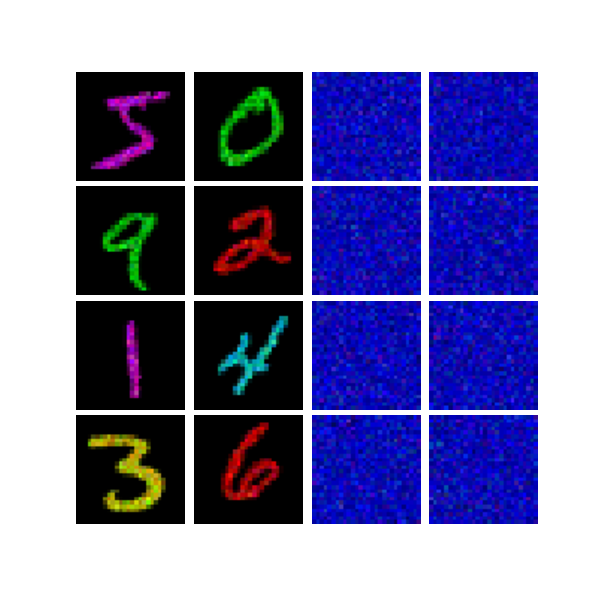
\includegraphics[width=.2\textwidth]{img/cav_viz}
%    %\caption{Caption}
%    \label{fig:big}
%\end{figure}

\vspace{8mm}

\alert{Sanity Check: Test Accuracies of Balanced and Biased Models}
\begin{figure}%
    \centering
    \subfloat[Accuracy of model trained on color-balanced data set and tested on color-biased data sets]{{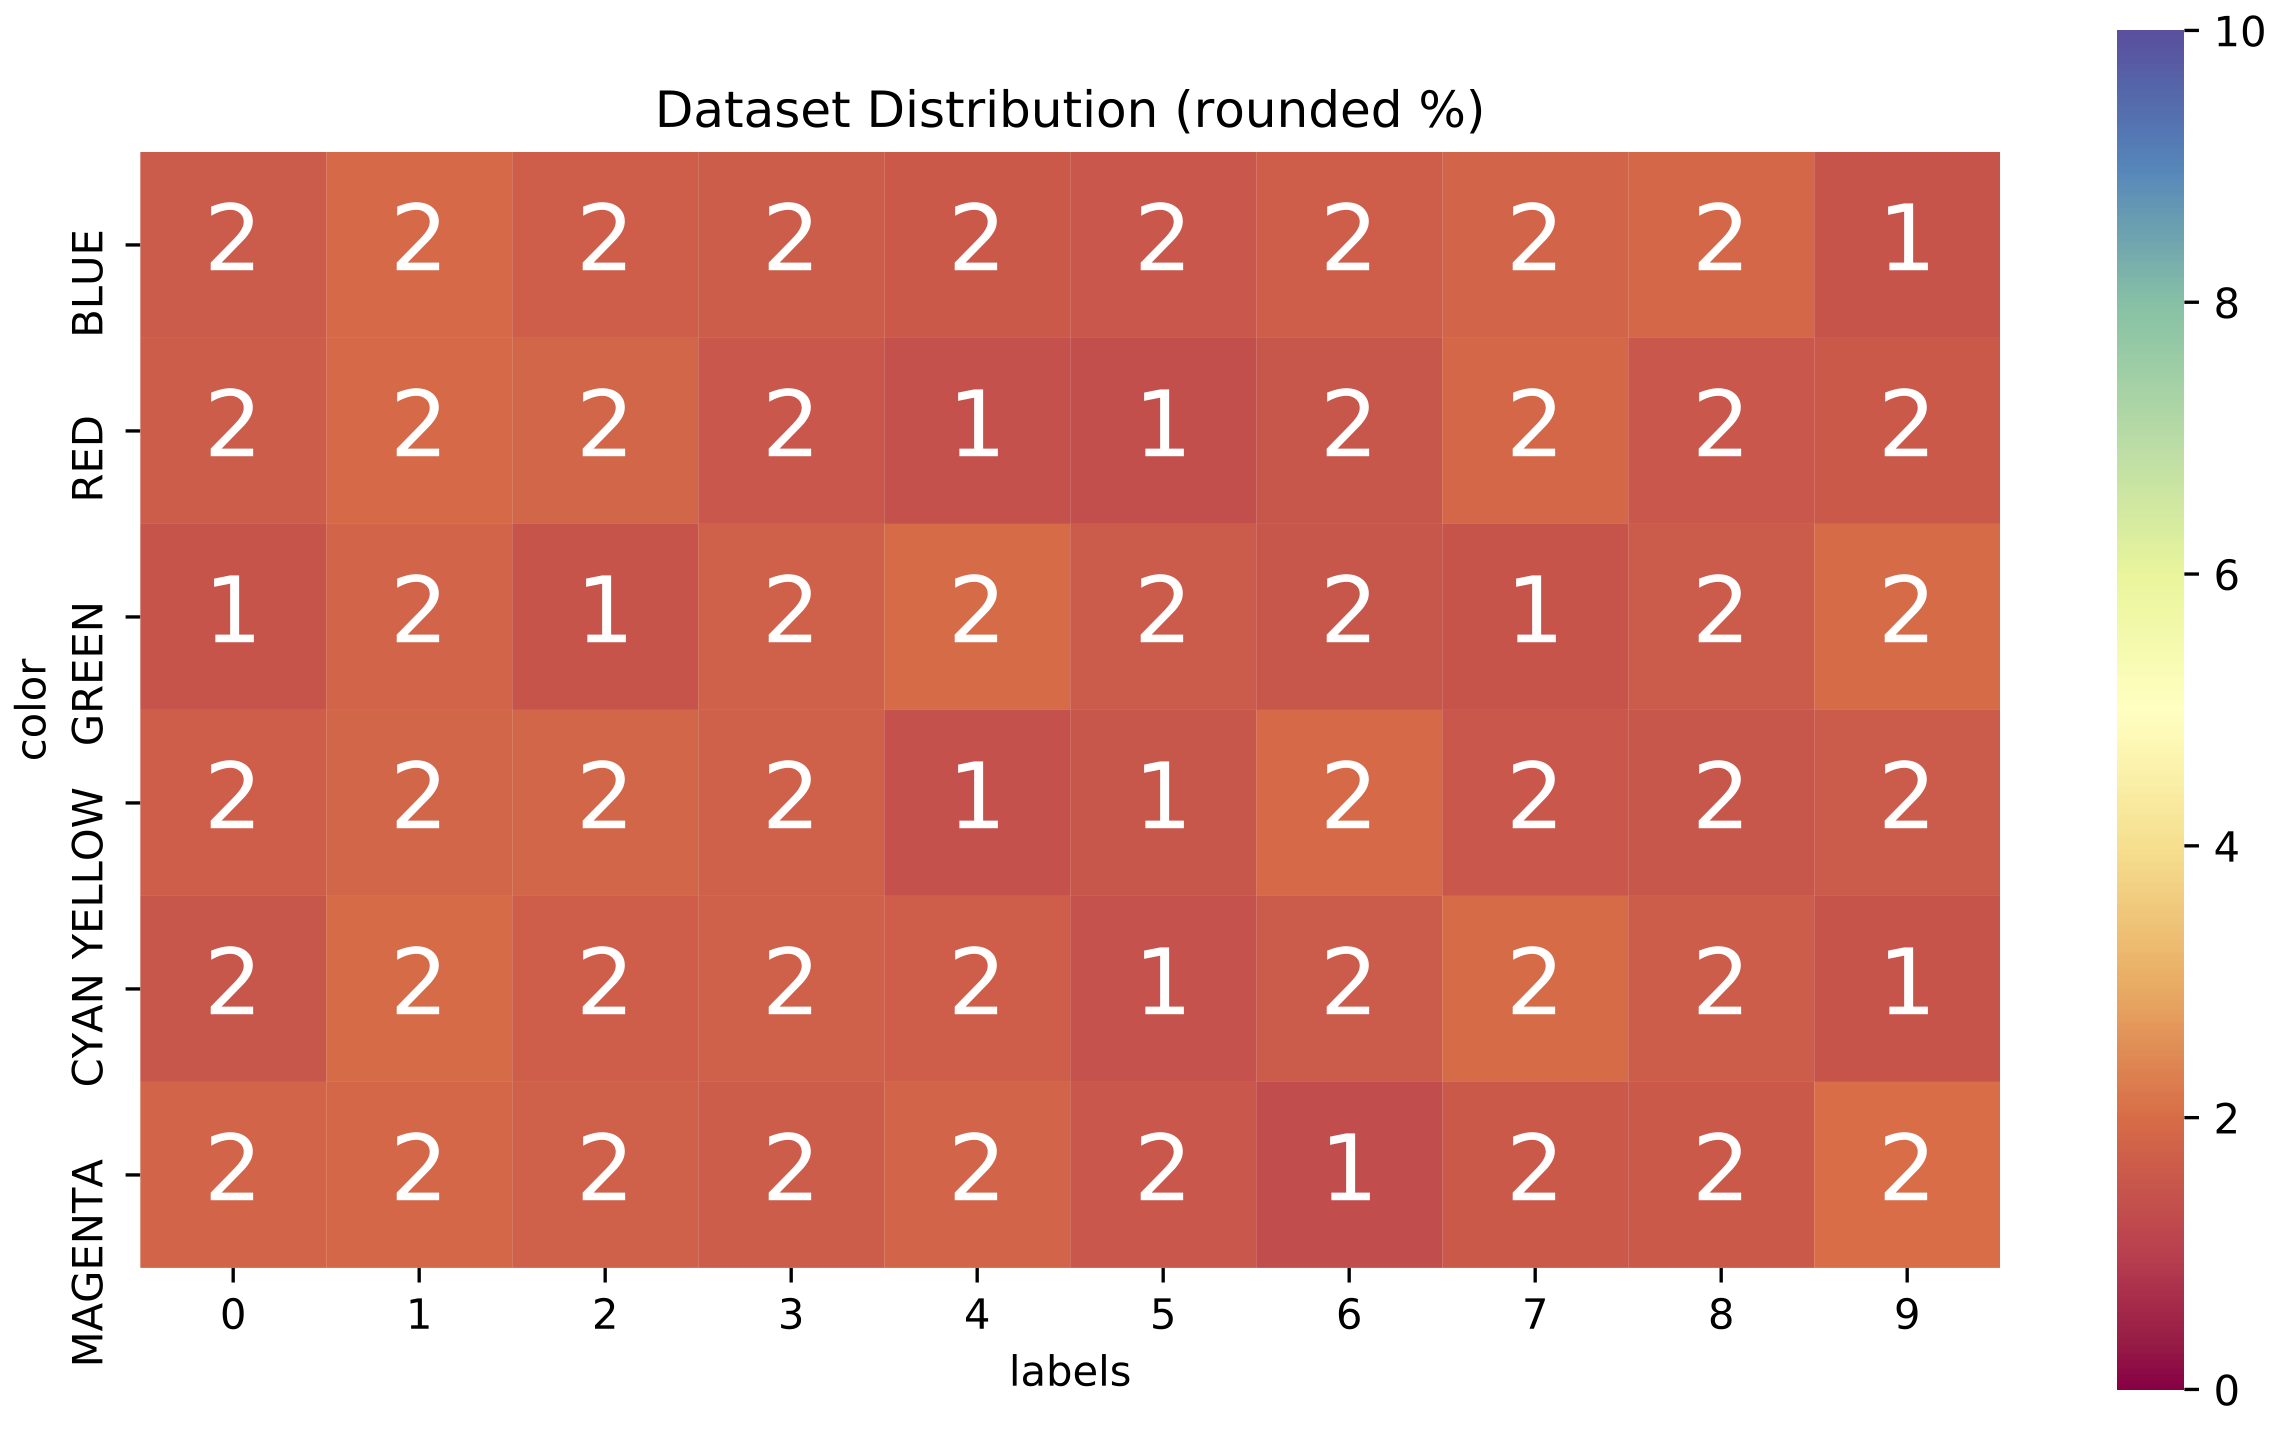
\includegraphics[width=.4\textwidth, backgroundcolor=white]{img/data_distr_balanced_test_new2} }}%
    \qquad
    \subfloat[Accuracy of model trained and tested on color-biased data-set]{{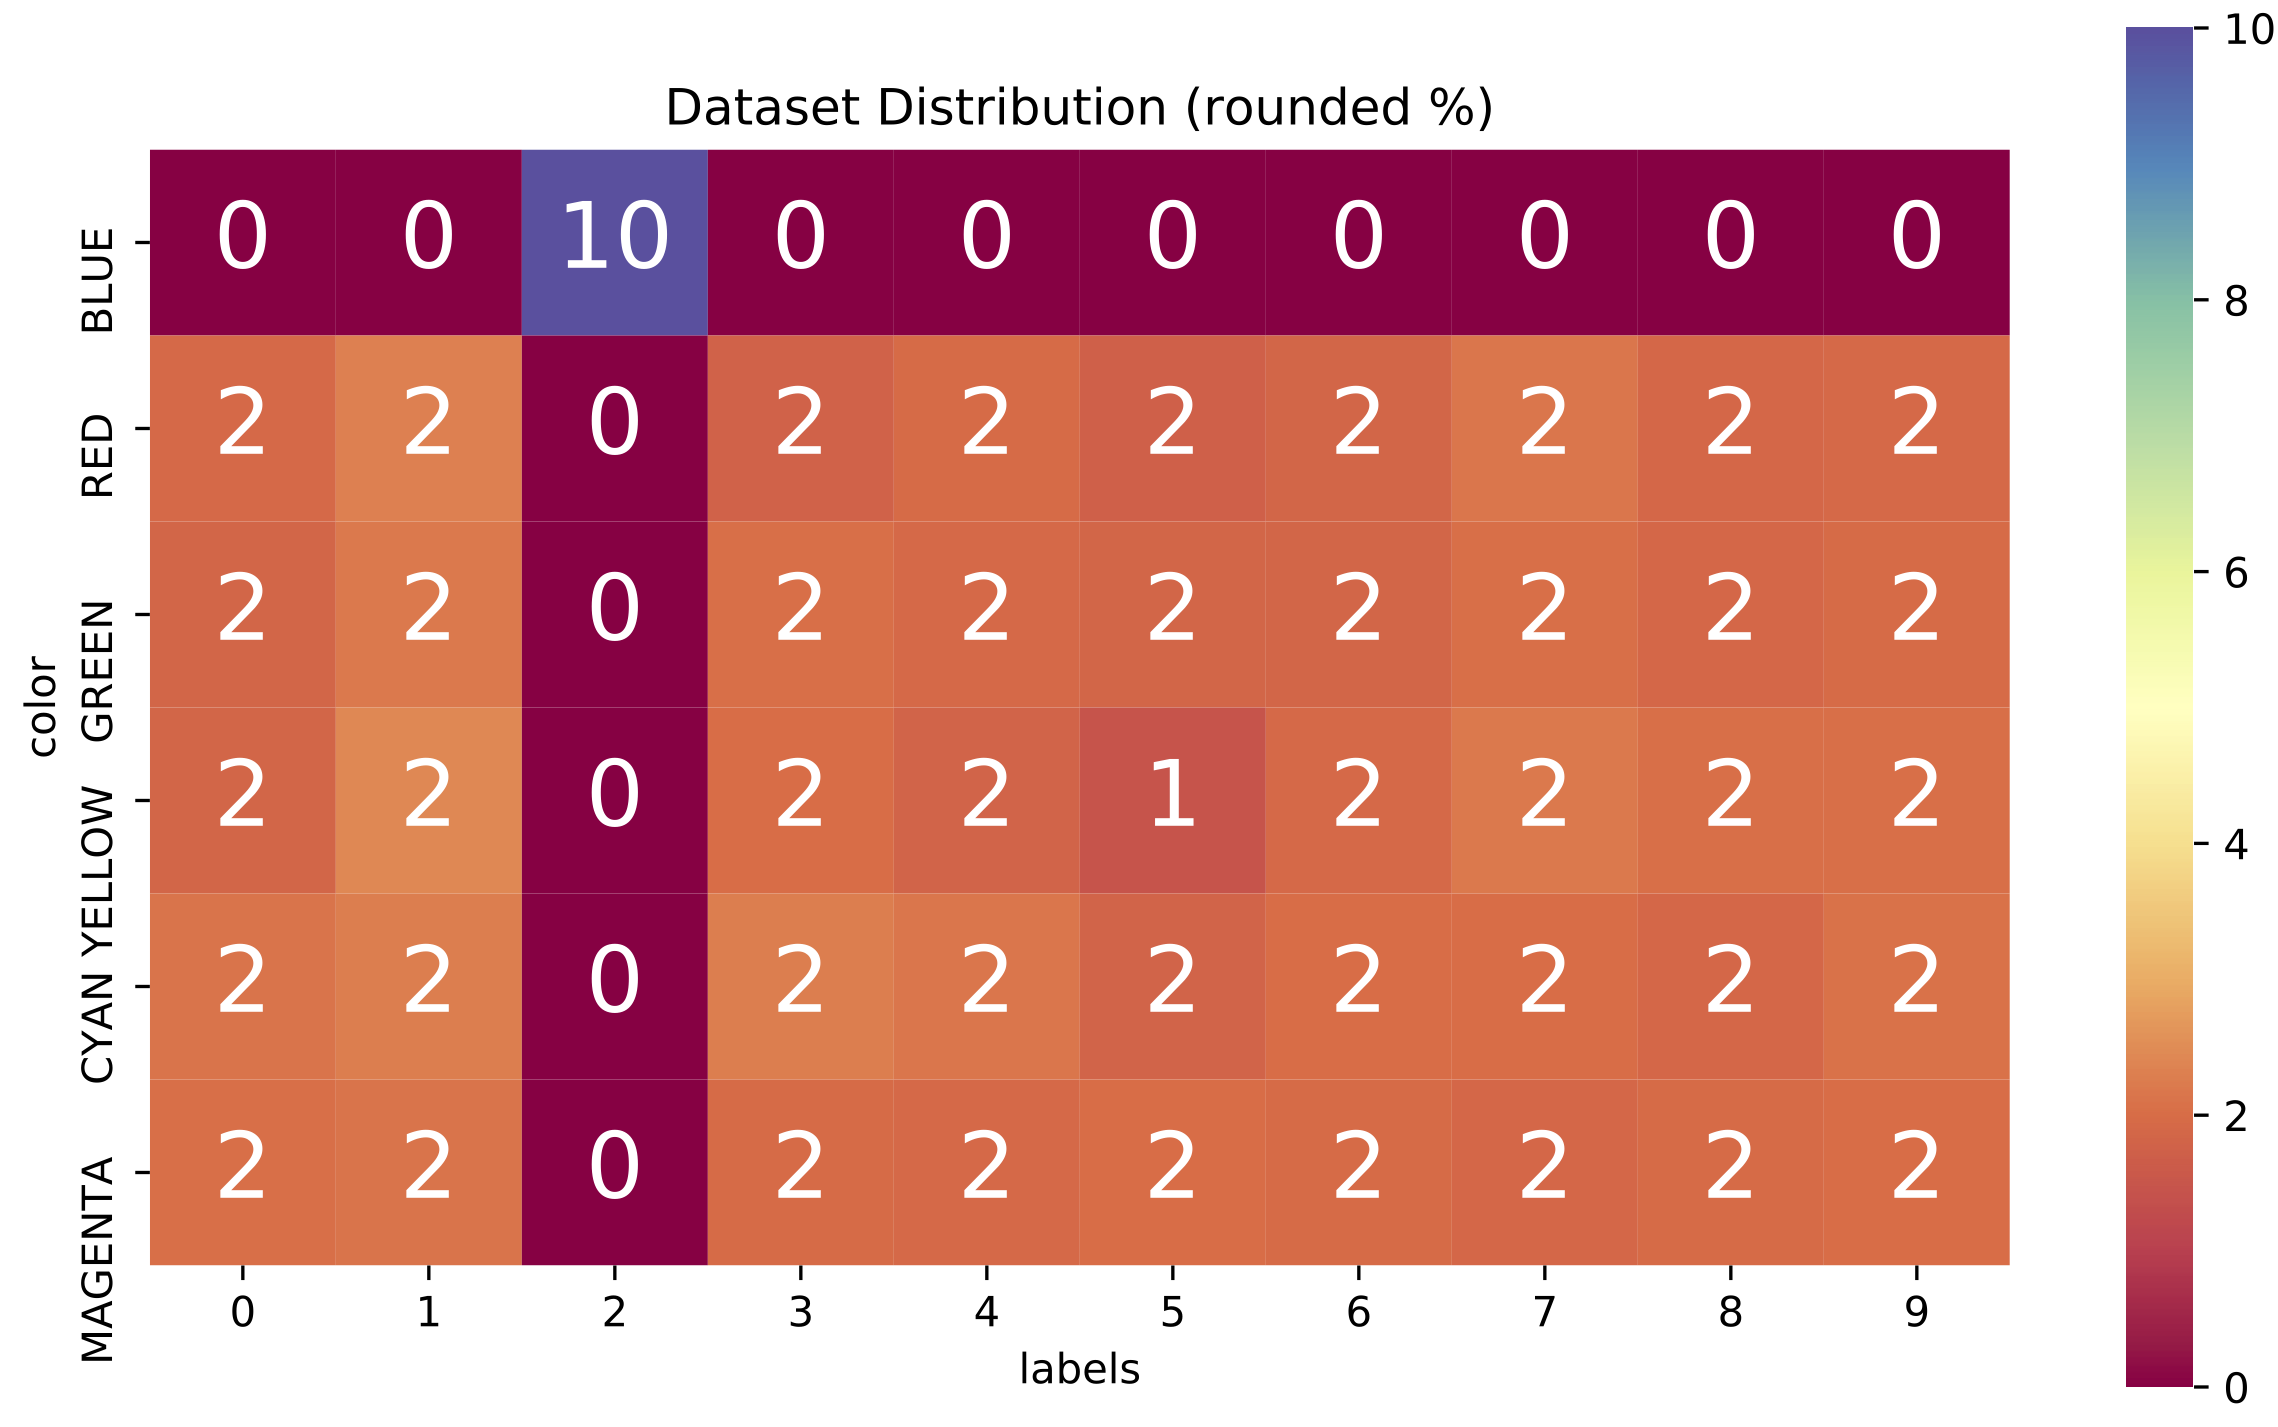
\includegraphics[width=.4\textwidth]{img/data_distr_blue2_test_new2} }}%
%    \caption{2 Figures side by side}%
    \label{fig:example}%
\end{figure}

\vspace{8mm}

\alert{Results}

\vspace{8mm}

\begin{figure}%
    \centering
    \subfloat{{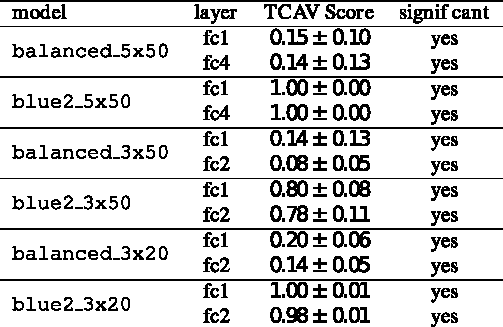
\includegraphics[width=.4\textwidth]{img/table1} }}%
    \qquad
    \subfloat{{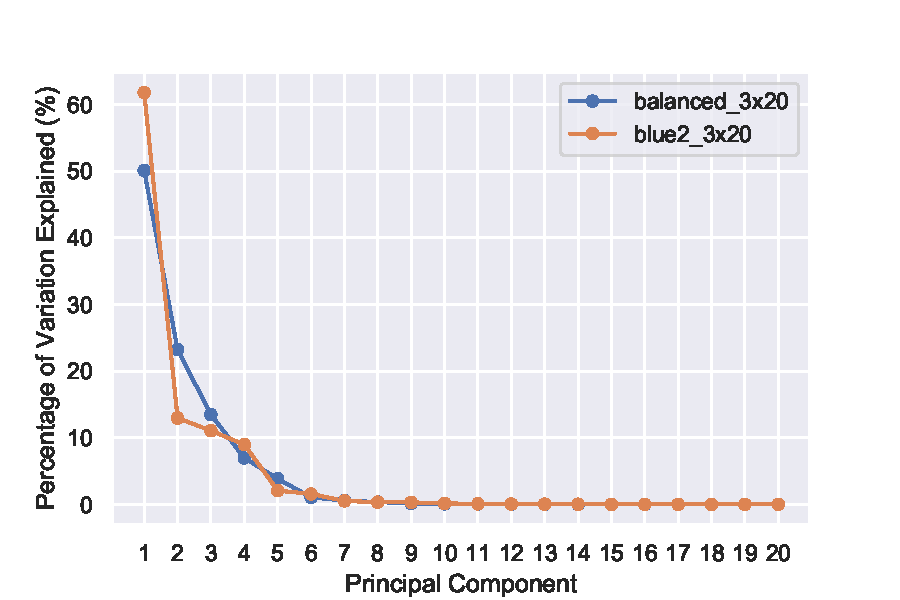
\includegraphics[width=.4\textwidth]{img/scree_plot} }}%
    \qquad
    \caption{\textcolor{cardinal}{(a)} TCAV scores and $p$-values for testing the concept blue for class 2. A significant test indicates that there is sufficient evidence to suggest that the concept blue is relevant in the classification of the class 2. \textcolor{cardinal}{(b)} Percentage of variation explained by the principal components of the CAVs for the concept blue, for the models trained on the color-balanced and blue-biased data sets.}%
    \label{fig:example}%
\end{figure}

\end{paddedBlock}
%\vspace{3mm}
\end{textblock}


\begin{textblock}{\colwidth}(\thirdcolpos,\vstartCols)

%\begin{paddedBlock}

%\
%$\hat{y}=\mathrm{GCN}(\hat{A}, X)$

%\end{paddedBlock}

\begin{paddedBlock}{Approach \#2: Formal Methods}
%\vspace{8mm}

%\vspace{8mm}
\alert{Properties}

\begin{itemize}
\item \textbf{Input sets:}
	\begin{itemize}
	\footnotesize{
	\item $\mathcal{X}_1 = \{ x \in \mathcal{D}_{\vec x} \mid 0 \leq r(x) \leq 25,  0 \leq g(x) \leq 25, 150 \leq b(x) \leq 255 \}$, where $r(x)$, $g(x)$, and $b(x)$ correspond to the red, green, and blue channels of image $x$, respectively. 
	\item $\mathcal{X}_{2,r} = \{x \in \mathcal{D}_{\vec x} \mid \left  \| x - x_0 \right \|_{\infty} \leq r \}$, where $x_0$ is an arbitrary training image of a blue $2$. This set corresponds to a hypercube centered on a blue 2 with radius $r$.
    }
	\end{itemize}
\item \textbf{Output sets:}
	\begin{itemize}
	\footnotesize{
	\item $\mathcal{Y}_{\pm v, l} = \{ y \in \mathcal{D}_{\vec y_l} \mid \pm y^{T}v \geq 0 \}$. This set corresponds to the positive ($+$) or negative ($-$) halfspace defined by the vector $v$ in the space of the activations of layer $l$. 
    }
	\end{itemize}
\end{itemize}

\vspace{8mm}

\alert{Results}
 
\begin{table}
\centering
\scalebox{0.7}{
\begin{tabular}{lcccc}
\hline
\textbf{Property \#} & \textbf{network} &  \textbf{in/out sets} &   \textbf{algorithm}  &  \textbf{result} \\ \hline 
\multirow{2}{*}{1} & \texttt{blue2\_5x50} & $\mathcal{X}_1$/$\mathcal{Y}_{+ \text{PC1}, \text{fc4}}$ &  NSVerify &  violated \\
                   & \texttt{balanced\_5x50} & $\mathcal{X}_1$/$\mathcal{Y}_{+ \text{PC1}, \text{fc4}}$ &  NSVerify &  violated \\
\hline
\multirow{2}{*}{1.1} & \texttt{blue2\_5x50} & $\mathcal{X}_1$/$\mathcal{Y}_{+ \text{mean}, \text{fc4}}$ &  NSVerify &  violated \\
                   & \texttt{balanced\_5x50} & $\mathcal{X}_1$/$\mathcal{Y}_{+ \text{mean}, \text{fc4}}$ &  NSVerify &  violated \\
\hline

\multirow{2}{*}{2} & \texttt{blue2\_3x20} & $\mathcal{X}_1$/$\mathcal{Y}_{+ \text{PC1}, \text{fc2}}$ &  Reluplex &  violated \\
                   & \texttt{balanced\_3x20} & $\mathcal{X}_1$/$\mathcal{Y}_{+ \text{PC1}, \text{fc2}}$ &  Reluplex &  violated \\
\hline
\multirow{2}{*}{2.1} & \texttt{blue2\_3x20} & $\mathcal{X}_1$/$\mathcal{Y}_{+ \text{mean}, \text{fc2}}$ &  Reluplex &  violated \\
                   & \texttt{balanced\_3x20} & $\mathcal{X}_1$/$\mathcal{Y}_{+ \text{mean}, \text{fc2}}$ &  Reluplex &  violated \\
\hline
\multirow{2}{*}{3} & \texttt{blue2\_5x50} & $\mathcal{X}_{2,5}$/$\mathcal{Y}_{+ \text{PC1}, \text{fc4}}$ &  NSVerify &  unknown \\
                   & \texttt{balanced\_5x50} & $\mathcal{X}_{2,5}$/$\mathcal{Y}_{+ \text{PC1}, \text{fc4}}$ &  NSVerify &  unknown \\
\hline
\multirow{2}{*}{3.1} & \texttt{blue2\_3x20} & $\mathcal{X}_{2,5}$/$\mathcal{Y}_{+ \text{PC1}, \text{fc2}}$ &  NSVerify &  holds \\
                   & \texttt{balanced\_3x20} & $\mathcal{X}_{2,5}$/$\mathcal{Y}_{+ \text{PC1}, \text{fc2}}$ &  NSVerify &  violated \\
\hline
\end{tabular}
}
\caption{Results of formal verification experiments for various networks, input and output sets, and algorithms. If the result is violated, this indicates that $\vec x \in \mathcal{X} \nRightarrow \vec y = \vec f(\vec x) \in \mathcal{Y}$.}
\label{table:properties}
\end{table}

\alert{Analysis}

\begin{itemize}
  \item Property 3.1 indicates that the concept blue has a significant impact in the classification output of a $2$.
  \item If the methodology is correct, it would appear that blue is relevant for both networks trained on color-balanced and color-biased data sets. Perhaps the tests in TCAV are not sufficient to identify spurious CAVs.
\end{itemize}

\end{paddedBlock}


\begin{paddedBlock}{References}
\footnotesize{[1] G. Katz, C. Barrett, D. L. Dill, K. Julian, and M. J. Kochenderfer. Reluplex: An efficient smt solver for verifying deep neural networks. In International Conference on Computer Aided Verification, pages 97–117. Springer, 2017}

\footnotesize{[2] B. Kim, M. Wattenberg, J. Gilmer, C. J. Cai, J. Wexler, F. B. Viegas, and R. Sayres. Interpretability beyond feature attribution: Quantitative testing with concept activation vectors (tcav). In ICML, 2018}

%\footnotesize{[3] Y. LeCun, C. Cortes, and C. Burges. Mnist handwritten digit database. AT&T Labs [Online]. Available: http://yann. lecun. com/exdb/mnist, 2:18, 2010}

\footnotesize{[3] C. Liu, T. Arnon, C. Lazarus, C. Barrett, and M. J. Kochenderfer. Algorithms for verifying deep neural networks. CoRR, abs/1903.06758, 2019}

\end{paddedBlock}
\end{textblock}


%%%%%%%%%%%%%%%%%%%%%%%%%
%%%%%%%%%%%%%%%%%%%%%%%%%
%% BOTTOM ROW
%%%%%%%%%%%%%%%%%%%%%%%%%
%%%%%%%%%%%%%%%%%%%%%%%%%

%\begin{textblock}{\fullwidth}(2,\bottomblockstart)
%\begin{paddedBlock}[0.98\linewidth]{Acknowledgements}

%In case you need it, you can do this too

%\end{paddedBlock}
%\end{textblock}

\end{frame}
\end{document}
